\def\allfiles{}
\documentclass{package/fancy-book}
\setlength{\parindent}{2em}
\usepackage[UTF8]{ctex}
%%%%%%%%%% Default Package %%%%%%%%%%%%%
\usepackage{package/color-env}
\usepackage{package/quiver}
\usepackage{background}
\usepackage[object=vectorian]{pgfornament} %% used in title.tex
\usepackage{calligra} %%% (optional) to make the Title text beautiful 
\usepackage{lipsum}  %% for dummy text 
\usepackage{amssymb,amsmath,amsfonts}  %%% for maths
\usepackage{datetime}

%%%%%% Optional Packages %%%%%%%
\usepackage{lettrine} %% for nice looking 
\usepackage{GoudyIn} %% first Letter of the paragraph
\renewcommand{\LettrineFontHook}{\color{black}\GoudyInfamily{}}
\LettrineTextFont{\itshape}
\setcounter{DefaultLines}{3}%
%%%%%%%%%%%%%%%%%%%%%%%%%%%%%%%%%%%%%
\usepackage{datetime2}
\usepackage{fourier-orns}
\newcommand{\ornamento}{\vspace{2em}\noindent \textcolor{darkgray}{\hrulefill~ \raisebox{-2.5pt}[10pt][10pt]{\leafright \decofourleft 
\decothreeleft  \aldineright \decotwo \floweroneleft \decoone   \floweroneright 
\decotwo \aldineleft\decothreeright \decofourright \leafleft} ~  \hrulefill \\ \vspace{2em}}}



%%%% Bibliography %%%%%%%%%
% Required packages are included in notes class
% Can be tweaked in the notes.cls file itself
\addbibresource{resource/references.bib}
\includeonly{title,1,2,3}
\begin{document}
\begin{titlepage}

%%%%%%%%%%%%%%%%%%%%%%%%%%%%%%%%%%%% Inspired From  %%%%%%%%%%%%%%%%%%%%%%%%%%%%%%%%%%%%%%%%%%%%%%%%% 
%%%%  https://www.reddit.com/r/LaTeX/comments/j9d739/hello_world_in_latex_is_a_lot_cooler/   %%%%%
%%%%%%%%%%%%%%%% If this doesn't look nice then you may remove it %%%%%%%%%%%%%%%%%%%%%%%%%%

\backgroundsetup{
scale=1,
opacity=1,
angle=0,
color=black,
contents={
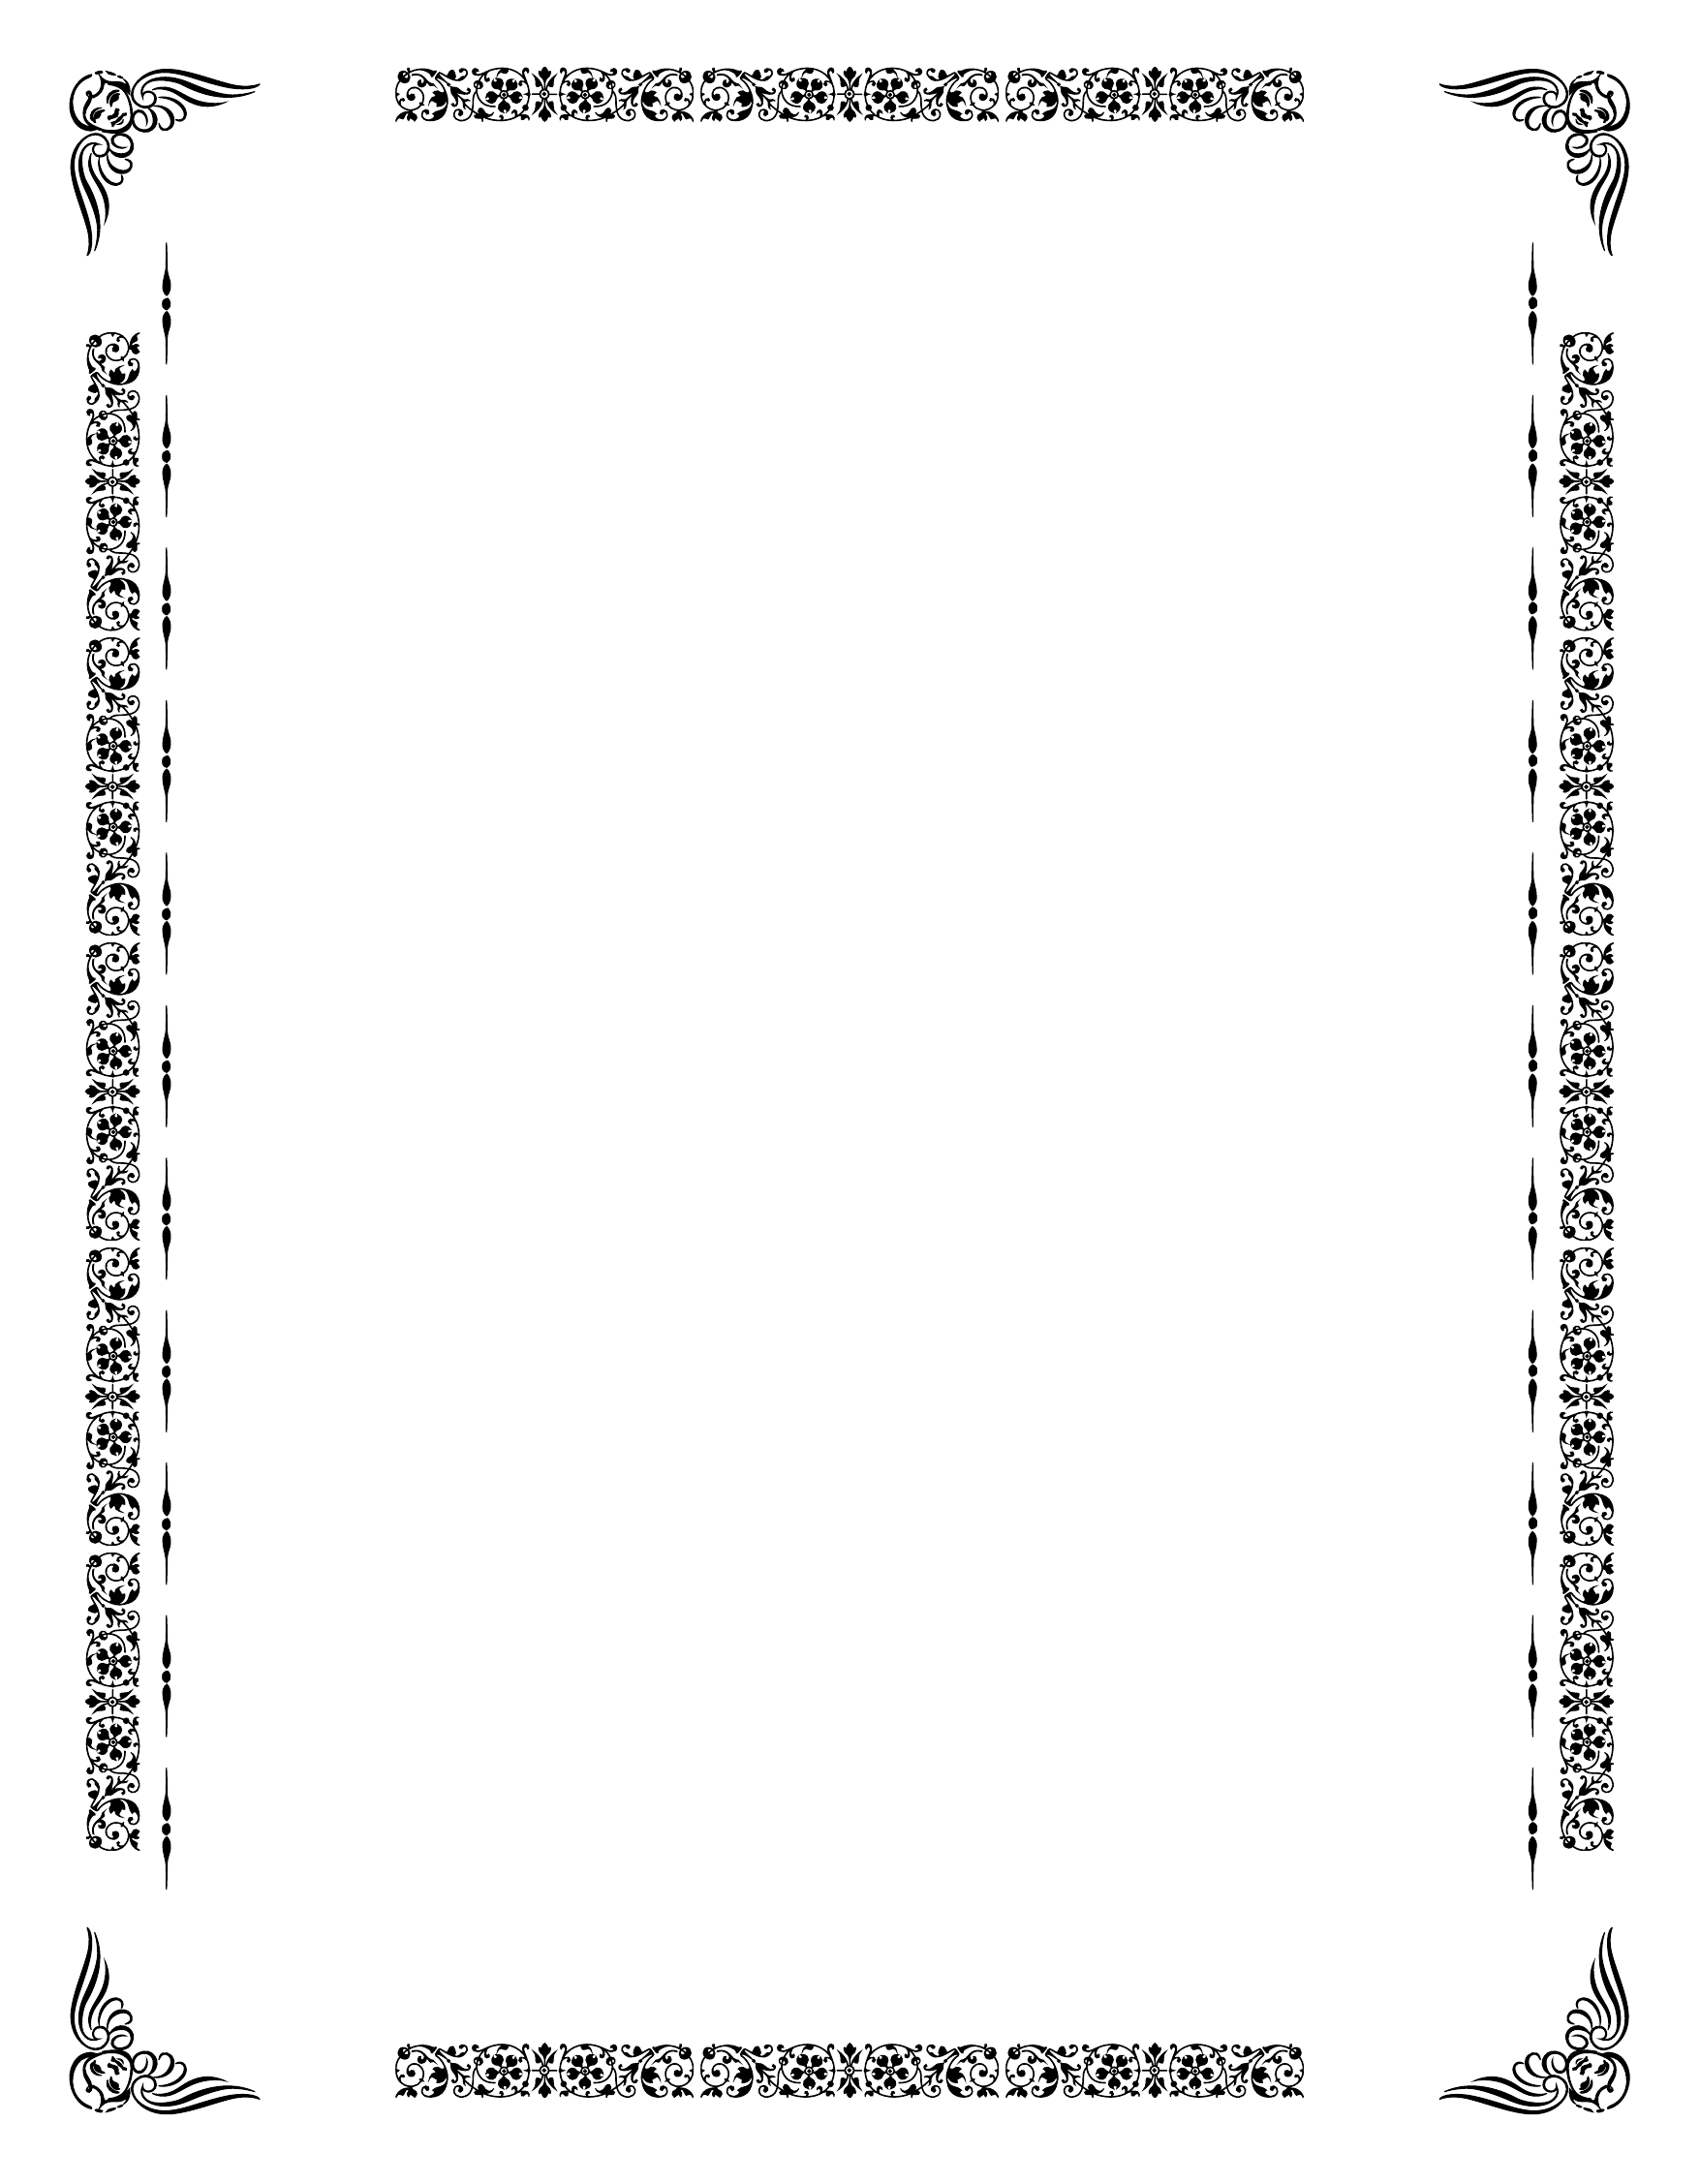
\begin{tikzpicture}[color=black, every node/.style={inner sep= 15pt}]
\node (NW) [anchor=north west] at (current page.north west){\pgfornament[width=2.5cm] {131}};
\node (NE) [anchor=north east] at (current page.north east){\pgfornament[width=2.5cm, symmetry=v]{131}};
\node (SW) [anchor=south west] at (current page.south west){\pgfornament[width=2.5cm, symmetry=h]{131}};
\node (SE) [anchor=south east] at (current page.south east){\pgfornament[width=2.5cm, symmetry=c]{131}};
\foreach \i in {-4,0,4}
\node[anchor=north,xshift=\i cm] at (current page.north){\pgfornament[scale=0.25,symmetry=v]{71}};
\foreach \i in {-4,0,4}
\node[xshift=\i cm, yshift=32.25 pt] at (current page.south){\pgfornament[scale=0.25,symmetry=v]{71}};
\foreach \i in {-8,-4,0,4,8}
\node[yshift=\i cm, xshift=32.25pt, rotate=90] at (current page.west){\pgfornament[scale=0.25,symmetry=v]{71}};
\foreach \i in {-8,-4,0,4,8}
\node[yshift=\i cm, xshift=-32.25pt, rotate=90] at (current page.east){\pgfornament[scale=0.25,symmetry=v]{71}};
\foreach \i in {-11,-9,...,7,9}
\node[anchor=west, yshift=\i cm, xshift=52.25pt, rotate=90] at (current page.west){\pgfornament[scale=0.1]{80}};
\foreach \i in {-11,-9,...,7,9}
\node[anchor=east, yshift=\i cm, xshift=-52.25pt, rotate=-90] at (current page.east){\pgfornament[scale=0.1]{80}};
\end{tikzpicture}
}}

%%%%%%%%%%%%%%%%%%%%%%%%%%%%%%%%%%%%%%%%%%%%%%%%%%%%%%%%%%%%%%%%%%%%%%%%%%%%%%%%%%%%%%%%%%%%%%%%%%%%%%%%%%%%%%%%%%

\centering % Centre everything on the title page
		
\scshape % Use small caps for all text on the title page

\vspace*{\baselineskip} % White space at the top of the page

%------------------------------------------------
%	Title
%------------------------------------------------

\rule{\textwidth}{1.6pt}\vspace*{-\baselineskip}\vspace*{2pt} % Thick horizontal rule
\rule{\textwidth}{0.4pt} % Thin horizontal rule

\vspace{0.75\baselineskip} % Whitespace above the title

{\huge \calligra{\textbf{Note for Homological Algebra} }\\} % Title

\vspace{0.75\baselineskip} % Whitespace below the title

\rule{\textwidth}{0.4pt}\vspace*{-\baselineskip}\vspace{3.2pt} % Thin horizontal rule
\rule{\textwidth}{1.6pt} % Thick horizontal rule

\vspace{2\baselineskip} % Whitespace after the title block

%------------------------------------------------
%	Subtitle
%------------------------------------------------

\Huge{Morse理论笔记} 

\vspace*{3\baselineskip} % Whitespace under the subtitle



\vspace{0.5\baselineskip} 

{\scshape   \LARGE Edited by\\  颜成子游/南郭子綦} % Editor list
\vspace{0.2\baselineskip} 


\vfill 
\Large{最后一次编译时间:\DTMnow}
%------------------------------------------------
% Author
%------------------------------------------------

\begin{figure}[!h]
    \centering
    
\includegraphics[width = 3cm, height= 3cm]{resource/icon.png}%% include the university icon here
\end{figure}
\vspace{0.3\baselineskip} 

\end{titlepage}
\backgroundsetup{contents={}} %% to remove background and watermark from other pages
\tableofcontents

\quad
\newpage
这是笔者于2023年本科四年级下学期学习Morse理论的学习笔记。

我们假定大家拥有基础的微分几何知识和黎曼几何知识。

设$f$是流形$M$上的光滑函数。我们定义:称一个点$p\in M$是$f$的临界点(critical point),若诱导映射$f_*:T_pM \to T_{f(p)}R$是$0$映射。

在流形上我们最好用各种各样的局部坐标讨论。设$(U;x_i,1\leq i \leq n)$是$p$附近的一个局部坐标系,则临界点的定义可以写为:
\begin{align}
	\pa{f}{x^1}=\pa{f}{x^2}=\dots=\pa{f}{x^n}=0
\end{align}

此时$f(p)$称为$f$的临界值。

在临界点处$f$的性质有着与非临界值完全不同的性质。Morse理论则是研究临界点处,$M$本身拓扑性质的改变的理论。
\ifx\allfiles\undefined

	% 如果有这一部分另外的package,在这里加上
	% 没有的话不需要
	
	\begin{document}
\else
\fi
\chapter{黎曼曲面}
\section{黎曼曲面的定义:从解析延拓讲起}
在基础复变函数论中,我们曾经接触一类多值函数(如$f=z^{1/2}$).这类函数的特点是,对于自变量的某些取值,函数将给出多个取值.

在经典复分析中,我们采取的办法是寻找解析分支.例如对于函数$f=z^{1/2}$,只要任选一条从$0$出发的射线$\gamma$,就可以在$\C \setminus \gamma$上定义解析函数$z^{1/2}$.如果选取$\gamma$是$x$正方向轴,则函数$f(z)$在$\C \setminus \gamma$上可以给出一个解析分支:
\begin{align*}
	f(r e^{i2\pi t})=\sqrt{r}e^{i\pi t}, 0<t<1
\end{align*}

因此,从某种意义上讲,多值函数是若干个解析函数“粘起来”的结果.这些解析函数都只在$\C$的一个开域上有定义.这启发我们从局部的角度来研究复函数.

\subsection{解析开拓}
在本笔记中,我们将统一使用记号$\OO(U)$表示开集$U$上的全纯(解析)函数.
\begin{definition}
	设$D_1,D_2$是$\C$的两个开域且$D_1\cap D_2 \neq \emptyset$.选取$f \in \OO(D_1)$,$g \in \OO(D_2)$.若在$U_1\cap U_2$上$f,g$满足$f \equiv g$,则成$(f,D_1)$和$(g,D_2)$互为对方的解析延拓.

	类似的,也可以在$D_1\cap D_2=\emptyset$的情况下定义解析延拓.若存在开集族$B_1,\dots,B_N$使得$B_1=D_1,B_N=D_2$,且存在$f_1,\dots,f_N$使得$f_i \in \OO(B_i)$且$(f_i,B_i)$与$(f_{i+1},B_{i+1})$互为解析延拓,$f_1=f,f_N=g$.则称$(f,D_1)$与$(g,D_2)$互为解析延拓.
\end{definition}

有时候我们希望解析延拓的方式“沿着”某根曲线$\gamma$前进.此时,只需要求$\gamma$与$D_1,D_2$相交,且定义中的开集族$B_1,\dots,B_N$是$\gamma$的一个开覆盖即可.根据唯一性定理,沿着同一根曲线的解析延拓是唯一的.

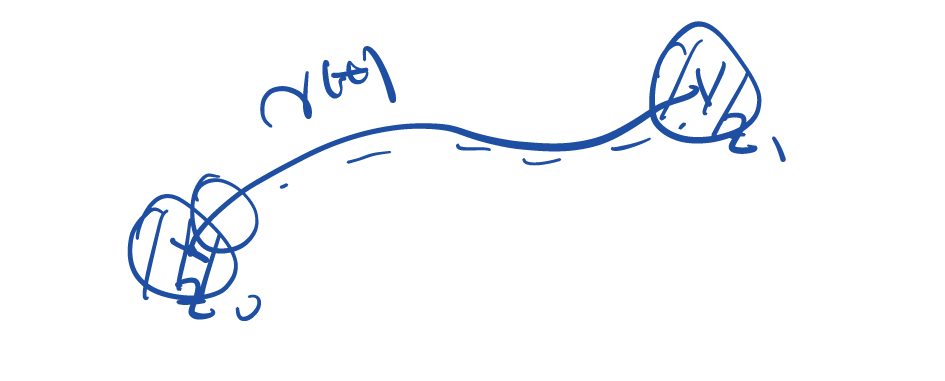
\includegraphics[scale=0.25]{resource/extension by lines.png}

有了上述概念,我们可以严格的定义多值解析函数.
\begin{definition}[多值解析函数]
	设$D$是$\C$上的开域(domain,即道路连通的开集),$f(z)$是$D$上的多值函数(对于$z$,$f(z)$是一个非空点集).若存在$z_0 \in D$,$B_R(z_0)$以及在$B_R(z_0)$上收敛的幂级数$P_0(z)$满足:
	\begin{enumerate}
		\item $P_0$在$D$中沿着以$z_0$为起点的任意曲线$\gamma$均可解析开拓.
		\item 当$z \in D$时,$f(z)=\{P(t)|P\text{为}P_0\text{沿着}D\text{中连接}z_0,z\text{的某曲线的解析开拓}\}$.
	\end{enumerate}
	
	即$f(z)$可由定义在$B_R(z_0)$上的$P_0(z)$解析延拓得到.此时,称$f(z)$为$D$上的\textbf{多值解析函数}.
\end{definition}

注意,这里的关键在于任何一个点$p$处,总存在一个小邻域$U$使得$f$在$U$上有单值解析分支.因此对于$z^{1/2}$而言,$0$不是$z^{1/2}$的解析点.(称为支点)

对于多值解析函数,我们有如下的单值性定理(Monodromy)
\begin{theorem}
	设$f$是开域$D \subset \C$上的多值解析函数.$z_0 \in D$,$w_0\in f(z_0)$.若$G$是$D$的一个单连通开集,且$z_0 \in G$,则$G$上必定有单值解析分支$g(z)$使得$g(z_0)=w_0$且$f(z)$可由定义在$G$上的$g(z)$解析延拓得到.
\end{theorem}
\begin{proof}
	互为解析延拓是等价关系,因此$f$可由$B_R(z_0)$处的幂级数$P_0(z)$解析延拓得到.若$G=\C$,则在复平面上$P_0$均可延拓,也即$P_0(z)$的收敛半径是$\infty$.从而自然存在一个单值解析分支.

   若$G \neq \C$,则根据黎曼映照定理,存在解析同构$\varphi:G \to V(0,1)$.从而$P_0 \circ \varphi^{-1}$是$V(0,\delta)$($\delta$是某个正数)上的解析函数.
   幂级数展开:
   \begin{align*}
	P(z)=\sum_{n=0}^\infty \frac{(P_0\circ \varphi^{-1})^{(n)}}{n!}z^n,\text{收敛半径}r>0
   \end{align*}

   如果$P(z)$的收敛半径$r \geq 1$,则可定义$g=P\circ \varphi$证毕.事实上,由于$P_0$在$G$上可解析开拓,从而$P$在$V(0,1)$上也可解析开拓,因此$r\geq 1$成立.
\end{proof}

通过上述讨论,我们不难发现局部研究解析函数的便利.然而,局部研究清楚后,我们必须转入“整体”的性质.下面的讨论并不是黎曼曲面严格的定义,而是对“Unramified Riemann Surface”的讨论.

设$U$是$\C$的一个开域.
\begin{definition}[解析函数芽]
	任取$p \in U$,考虑集合$\{(f,V)|f \in \OO(V),p \in V\subset U,V\text{是开集}\}$. 定义该集合上的等价关系:
\begin{align*}
	(f_1,V_1)\sim (f_2,V_2) ,\text{若存在}B_{\delta}(p)\subset V_1\cap V_2,\text{使得在}B_{\delta}(p)\text{有}f_1=f_2
\end{align*}
 \[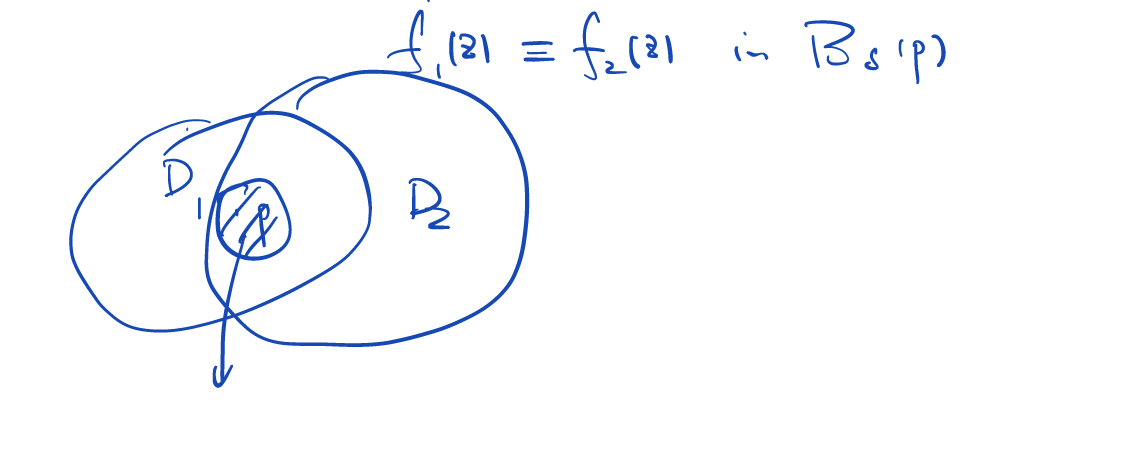
\includegraphics[scale=0.3]{resource/function germ.png}\]

  称上述集合商去该等价关系后得到的集合为$p$处的解析函数芽集.用$[f,p]$表示$(f,D)$的等价类.
\end{definition}

任何一个解析函数芽都意味着$p$处的一个开集合$U$以及$f \in \OO(U)$.同时,由定义不难验证,也给出了$p$处的一个函数值$f(p)$.

\begin{example}
	取$D=C^*$,$p=1$.$f(z)=1+\sum_{n=1}^\infty (-1)^{n-1}\frac{(2n-1)!!}{2^n}(z-1)^n$.

	不难验算,$f$实际上是$z^{1/2}$在$1$处的泰勒展开式.$[f,1]$给出了$1$处的某种函数结构.
\end{example}

\begin{definition}[Unramified Riemann Surface]
	定义:
	\begin{align*}
		\text{RS}(U,f_0,p_0):=\{[f,p]|p\in U,(f,B_{\delta}(p))\text{可由}(f_0,B_\delta(p_0))\text{解析延拓得到}\}
	\end{align*}
	给定该集合一个拓扑.定义$[f,D]:=\{[f,p]|p\in D\subset U,(f,D)\text{可由}(f_0,B_{\delta}(p_0))\text{在}U\text{中解析延拓得到}\}$.读者不难验证上述$[f,D]$给出的集族满足拓扑基的要求,我们定义$\text{RS}(U,f_0,p_0)$的拓扑由上述拓扑基给出.
\end{definition}
\begin{example}
	设$D=B_{1/2}(1)$.$f(z)=1+\sum_{n=1}^\infty (-1)^{n-1}\frac{(2n-1)!!}{2^n}(z-1)^n$.从上面的例子,$f$是$z^{1/2}$在$1$附近的展开.

	我们考虑$\text{RS}(C^*,f,1)$.

	沿着曲线$\gamma(t)=e^{i2\pi t},0\leq t\leq 1$解析延拓$f(z)$.$f(z)$变为:
	\begin{align*}
		g(z)=-1+\sum_{n=1}^\infty (-1)^{n-1}\frac{(2n-1)!!}{2^n}(z-1)^n
	\end{align*}

	从而绕一圈后$[f,D]\neq [g,D]$.

	同理,沿着曲线$\gamma(t)=e^{i2\pi t},0\leq t\leq 1$解析延拓$g(z)$,一圈后我们将重新得到$f(z)$.
\end{example}

我们大致可以感受到$\text{RS}(C^*,f,1)$的结构.形象地说,这一个由两个面交错粘在一起的得到的东西.

接下来我们考虑一般意义下RS的拓扑性质.
\begin{proposition}
	上述集合在上述拓扑下拥有的拓扑性质有:
	
	1.道路连通.

	2.Hausdorff.

	3.“局部维度”都是2.
\end{proposition}
笔者相信这三个论题是很好的点集拓扑与复变函数习题,因此不赘述证明.

\begin{remark}
	除开拓扑上的观察,我们还可以写出两个典范(canonical)的连续映射.

	Projection \quad $\pi:\text{RS}(U,f_0,p_0) \to U,[f,p]\mapsto p$.

	Function \quad $F:\text{RS}(U,f_0,p_0) \to \C,[f,p]\mapsto f(p)$
\end{remark}
\subsection{黎曼曲面}
我们现在严格的阐述黎曼曲面的定义.在此之前,我们做一个声明.

\textbf{在之后的笔记中,我们将统一使用$\ii$表示虚数单位.$i,j$这样的字母容易与指标产生混淆.}
\begin{definition}[黎曼曲面]
	设$M$是具有可数拓扑基的Hausdorff空间.若$M$上存在开覆盖$\{U_\alpha\}_{\alpha \in \Gamma}$以及定义在每个开集$U_\alpha$上的连续映射$\varphi_\alpha:U_\alpha \to \C$满足:
	\begin{enumerate}
		\item $\varphi_\alpha(U_\alpha)$是$\C$的开集,且$\varphi_\alpha$是给出$U_\alpha$与$\varphi_\alpha(U_\alpha)$的同胚.
		\item 若$U_\alpha \cap U_\beta \neq \emptyset$,则转移映射(transition map)$\varphi_\alpha \circ \varphi_{\beta}^{-1}:\varphi_\beta(U_\alpha \cap U_\beta) \to \varphi_\alpha(U_\alpha \cap U_\beta)$是解析映射.
	\end{enumerate}
	则称$M$是一个\textbf{黎曼曲面(Riemann Surface)}.同时,称$\{U_\alpha,\varphi_\alpha\}$是$M$上的\textbf{地图册(alts)}.
\end{definition}
粗略的说,黎曼曲面就是用解析的转移映射将若干个$\C$上的开集粘贴起来而得到的几何对象.如果读者熟悉微分流形,会发现这里的定义与微分流形的定义几乎完全一致,只是这里我们要求$M$局部上与$\C$上的某个开集同胚,而不是$\R^n$.
\begin{remark}
	定义中的“$\C$的开集”不能替换为$\C$.因为$\C$与$\C$上的单连通开集不一定可以解析同构(黎曼映照定理)
\end{remark}
\begin{remark}
	把$\C$改为$\C^n$,上述定义就变成了复流形的定义.因而黎曼曲面实际上无非是一维的复流形.
\end{remark}
我们给出若干黎曼曲面的例子.它们将贯穿整篇note.

\begin{example}[平凡的例子]
	$\C$中的开集.
\end{example}
\begin{example}[二维球面$S^2$.]
    显然$S^2$满足黎曼曲面的拓扑要求.

	为了得到地图册,这里我们用最经典的球极投影.$S^2=\{(x_1,x_2,x_3)|x_1^2+x_2^2+x_3^2=1\}$.令$U=S^2\setminus \{(0,0,1)\}$,$V=S^2\setminus \{(0,0,-1)\}$.定义:
	\begin{align*}
		\varphi_U:U \to \C, (x_1,x_2,x_3)\mapsto \frac{x_1}{1-x_3}+\ii\frac{x_2}{1-x_3}\\
		\varphi_V:V \to \C,(x_1,x_2,x_3)\mapsto \frac{x_1}{1+x_3}+\ii\frac{x_2}{1+x_3}
	\end{align*}

	球极投影的讨论告诉我们$\varphi_U,\varphi_V$都是同胚.再考虑转移映射$\varphi_V \circ \varphi_U^{-1}$的解析性:
   \begin{align*}
	\varphi_V \circ \varphi_U^{-1}:\varphi_U(U\cap V)\to \varphi_V(U\cap V),z \mapsto w=\frac{1}{z}
   \end{align*}

   因此$S^2$是一个黎曼曲面.
\end{example}
\begin{example}[射影直线$\PP^1$]
	类似于实射影空间,我们可以定义复的情况.考虑集合$\C^2\setminus\{0\}$,我们定义等价关系$\sim$:
	\begin{align*}
		z=(z_1,z_2)\sim w=(w_1,w_2) \Leftrightarrow \exists \lambda \in \C^*,z=\lambda w
	\end{align*}
	即$z$和$w$在同一条复直线上.

	定义$\PP^1:=\C^2\setminus\{0\}/\sim$.用$[z_1,z_2]$表示$(z_1,z_2)$所处的等价类.拓扑上,我们使用商拓扑.不难验证$\PP^1$是具有可数拓扑基的Hausdorff空间.

   接下来考虑地图卡.令$U=\{[z_1,z_2]|z_1\neq 0\}$,$V=\{[z_1,z_2]|z_2\neq 0\}$.定义$\varphi_U:U \to \C,[z_1,z_2]\mapsto z_2/z_1,\varphi_V:V \to \C,[z_1,z_2]\mapsto z_1/z_2$.不难验算,这是两个同胚的映射.

   最后考虑转移映射.在$U\cap V$上,转移映射可以写为:$z\mapsto 1/z$.因此这是一个解析的映射.
\end{example}

细心的读者肯定发现了上述两个例子有着非常强的相同性.事实上,$S^2$和$\PP^1$是同构的两个黎曼曲面.当然,我们首先要定义同构.

\begin{definition}[全纯(holomorphic)映射]
	设$M,N$是两个黎曼曲面,$f:M \to N$是连续映射.若对于任意$x \in M$,都存在$x \in U_\alpha\subset M,f(x)\in V_\beta \subset N$满足:
	\begin{align*}
		\phi_\beta \circ f \circ \varphi_\alpha^{-1}:\varphi_\alpha(\hat{U_\alpha}) \to \phi_\beta(V_\beta)
	\end{align*}
	是全纯函数,则称$f$是$M,N$之间的全纯映射.其中$\hat{U_\alpha}$表示使得上述映射有意义的$U_\alpha$子集.
    \[
	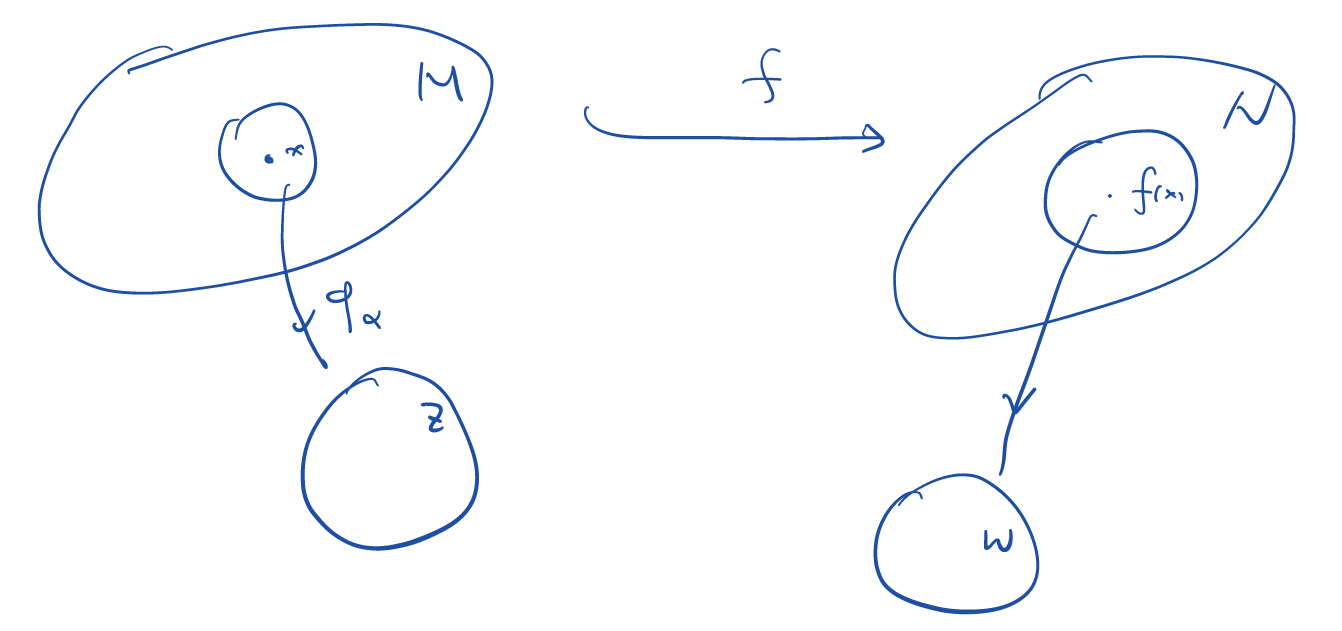
\includegraphics[scale=0.3]{resource/holomorphic map.jpg}\]
\end{definition}

\begin{definition}[双全纯(biholomorphic)映射]
	设$M,N$是黎曼曲面.若存在全纯映射$f:M \to N,g:N \to M$满足$f \circ C=\mathrm{id}_N,g\circ f=\mathrm{id}_M$,则称$M,N$是\textbf{双全纯等价}的黎曼曲面,$f,g$均为\textbf{双全纯映射}.
\end{definition}
\begin{example}
	$S^2$与$\PP^1$是双全纯等价的黎曼曲面.请读者尝试写出两者之间的双全纯映射.
\end{example}
\section{复分析回顾}

回忆一个定义:有理函数$R(z)=\dfrac{\mathrm{Polynomial}}{\mathrm{Polynomial}}$.有理函数是最简单的亚纯函数.
\begin{proposition}
	复平面上的亚纯函数的极点一定是孤立的.
\end{proposition}
\begin{proof}
	反证法.设$\{z_i\}$是一列$f$的极点,且拥有聚点$z_0$.同时$z_0$也是$f$的极点.

	取$\delta>0$使得$f(z)$在$\{|z-z_0|<\delta\}$上不为$0$(因为$|f|\to +\infty$).因此$1/f$在$\{|z-z_0|<\delta\}$是全纯函数.于是:
	\begin{align*}
		\frac{1}{f}=g(z)(z-z_0)^k,g(z_0)\neq 0
	\end{align*}

	再适当缩小$\delta$,使得$g$在$\{|z-z_0|<\delta\}$上也不为$0$.于是$\frac{1}{f}$在$\{|z-z_0|<\delta\}$上仅有$z_0$一个零点,矛盾于$z_j$都是$f$的极点!
\end{proof}

\begin{theorem}
	设$f$是亚纯函数.若$\infty$是$f$的可取奇点或者极点,则$f(z)$必定为有理函数.
\end{theorem}
\begin{proof}
	根据上述命题,存在$R>0$使得$f$在$\{R<|z|<\infty\}$上解析.设$\{z_1,\dots,z_n\}$是$f$在$\{|z|<R\}$的极点(孤立性保证有限),阶数为$k_1,\dots,k_n$.则:
	\begin{align*}
		f(z)=\sum_{l=1}^{k_j} \frac{C_j}{(z-z_j)^l}+P_j(z)=h_j(z)+P_j(z),\text{在}z_j\text{附近}
	\end{align*}
    
	由于$\infty$是可去奇点或者极点,则:
	\begin{align*}
		f(z)=\sum_{l=-\infty}^0 \frac{C_l}{z^{l}}+P(z),P(z)\text{是多项式(可以为}0)
	\end{align*}

	令$F=f-\sum_{j=1}^N h_j-g$,则$F(z)$是$\C$上的有界整函数.根据Liouville定理,$F(z)$是常数.

	因此$f=\sum_{j=1}^Nh_j+g$是有理函数.
\end{proof}
\begin{corollary}
	$\mathrm{Aut}(\C)=\{az+b|a \in \C^*,b\in \C\}$
\end{corollary}
\begin{proof}
	延拓到$\infty$.则$\infty$是极点或者可去奇点.从而$f$是多项式.由于$f^{-1}(0)$唯一,可知$f$是一次多项式.
\end{proof}
\begin{corollary}
	$\mathrm{Aut}(\C_\infty)=\{\dfrac{az+b}{cz+d}|ad-bc=1,a,b,c,d\in \C\}$
\end{corollary}
\begin{proof}
	分式线性变换一定是$C_\infty$的自同构.又因为自同构$f$是有理函数,从而$f$是多项式与多项式的比.由$0$原像和$\infty$原像唯一可得上下多项式均为一次.
\end{proof}
\section{黎曼曲面的更多例子}
本节我们讨论更多有意思的黎曼曲面.
\subsection*{黎曼环面}
\begin{definition}[Lattice Group]
	任取$w_1,w_2 \in \C^*$且实线性无关.定义群:
	\begin{align*}
		\Lambda:=\{nw_1+mw_2|n,m \in \Z\}
	\end{align*}
	群的运算是显而易见的.
\end{definition}
$\Lambda$可以自然的平移作用在$\C$上.我们考虑这个作用的商$C/\Lambda$.用$[z]$表示$z$的等价类.

从拓扑来说,$C/\lambda$显然同胚于环面$T^2$.从坐标卡来讲,在局部上$C/\lambda$总是一个未折叠的$\C$平面.因此$C/\Lambda$是一个黎曼曲面.

\begin{proposition}
	$\C/\Lambda$有全纯的自同构——平移.即$[z]\mapsto [z-z_0]$.
\end{proposition}
对于伸缩变换,$C/\Lambda$并不能有良好的定义.我们讨论的是两个黎曼环面的伸缩变换.
\begin{proposition}
	存在全纯映射:
	\begin{align*}
		f:\C/\la w_1,w_2\ra \to \C/\la 1,w_2/w_1\ra,[z]\mapsto [z/w_1]
	\end{align*}
    进一步的,$f$是双全纯映射.
\end{proposition}
因此,所有的黎曼环面都可以归结于一个上半平面的复数$z$.即总可以写为形式:
\begin{align*}
	C/\la 1,z\ra, \mathrm{Im}(z)>0
\end{align*}

然而不同的$z$是否给出不同的黎曼环面呢?答案是否定的.
\begin{proposition}
	若$\tau_1,\tau_2$是两个处于上半平面的复数,且$C/\la 1,\tau_1\ra \cong C/\la 1,\tau_2\ra$,则存在整数$a,b,c,d$满足$ad-bc=1$,使得
	\begin{align*}
		\tau_2=\frac{a\tau_1+b}{c\tau_2+d}
	\end{align*}
	换句话说,在相差一个$\mathrm{PSL}(2,\Z)$的元素的意义下,黎曼环面和上半平面有一一对应.
\end{proposition}
\begin{proof}
	注意到$\C \to \C/\Lambda$是一个开的覆叠映射.我们用一张图来表示这个结果.
    \[
	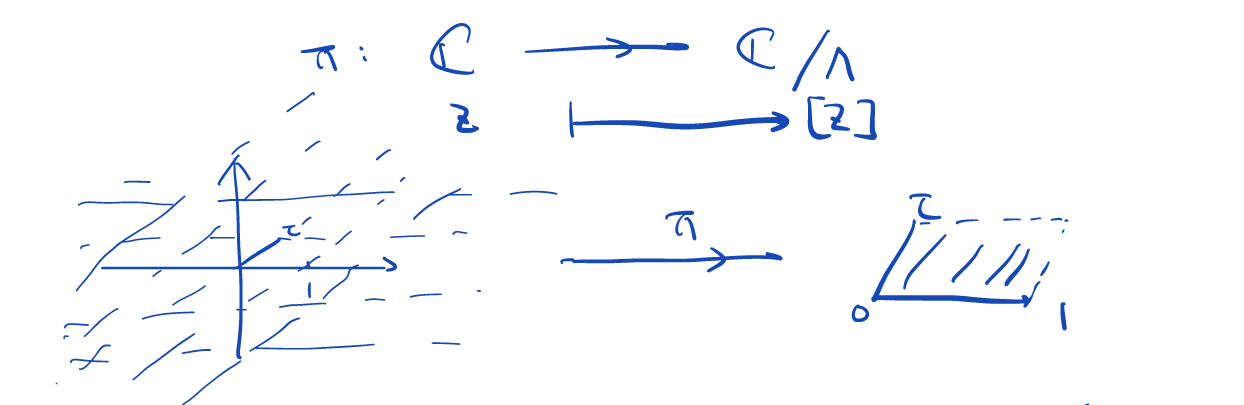
\includegraphics[scale=0.3]{resource/Riemann torus.png}
	\]

	假设同构映射是$f$.我们断言,存在一个提升映射$F$使得下面的交换图成立,并且$F(0)=0$,$F$是双全纯映射.
	\[\begin{tikzcd}
	\C && \C \\
	\\
	{\C/\la 1,\tau_1\ra} && {\C/\la 1,\tau_2\ra}
	\arrow["F", dashed, from=1-1, to=1-3]
	\arrow["{\pi_1}"', from=1-1, to=3-1]
	\arrow["{\pi_2}", from=1-3, to=3-3]
	\arrow["f"', from=3-1, to=3-3]
\end{tikzcd}\]
   
   如果断言成立,则$F=\gamma z,\gamma \in C^*$.并且$F$把格点映射为格点,从而$\gamma=F(1)=a+b\tau_2,\gamma \tau_1=F(\tau_1)=c+d\tau_2$.于是:
   \begin{align*}
	\tau_1=\frac{c+d\tau_2}{a+b\tau_2}
   \end{align*}

   同理,$\tau_2$也可写为类似的$\tau_1$的分式线性变换.根据双全纯,可知$a,b,c,d$必须满足$ad-bc=\pm 1$.根据$\tau_1$和$\tau_2$都是上半平面的点,可知:
   \begin{align*}
	ad-bc=1
   \end{align*}

   因此我们只需要说明$F$的存在性.根据平移变换,不妨假设$f([0])=[0]$.另一方面,根据覆叠映射的提升性质,在指定$F(0)=0$的情况下,存在唯一的$F$使得上述图交换.从而$F$存在.
\end{proof}
\subsection*{代数曲线}
接下里的例子是代数曲线.粗滤地说,我们考虑二元多项式在$\C^2$中的零点.

在此之前,我们需要先做一点理论性的准备.
\begin{theorem}[Implicit theorem]
	设$\Omega \subset \C^2$是开域,$F(z,w)\in \OO(\Omega)$(即$F$对两个分量都是全纯的).若$F(z_0,w_0)=0$,且$\pa{F}{w}(z_0,w_0)\neq 0$,则存在包含$z_0$的开集$U(z_0)\subset \C$,和一个单变量解析映射$w(z)\in \OO(U(z_0))$,满足$F(z,w(z))=0$在$U(z_0)$恒成立.
\end{theorem}
\begin{proof}
	因为$\pa{F}{w}(z_0,w_0)\neq 0$,于是存在$\delta>0$使得$\{|w-w_0|<\delta\}$内$F(z_0,w)$仅有$w_0$一个零点(重数为$1$)

	选取$0<\delta_0<\delta$使得$F(z_0,w)\neq 0,\forall \{|w-w_0|=\delta_0\}$.再选取$\epsilon>0$使得在$\{|z-z_0|<\epsilon\}\times \{|w-w_0|=\delta_0\}$上$F(z,w)\neq 0$.

	则对于每个固定的$z \in \{|z-z_0|<\epsilon\}$,有:
	\begin{align*}
		n(z)=\frac{1}{2\pi \ii}\int_{|w-w_0|=\delta_0} \frac{F_w(z,w)}{F(z,w)} dw=1(\text{根据连续性})
	\end{align*}

	因此存在唯一的$w$与$z$对应,且满足$F(z,w)=0$.记此$w$为$w(z)$.余下的事情是验证$w(z)$的解析性.解析性由下列引理保证.
\end{proof}
\begin{lemma}[]
	设$\Gamma$是闭曲线,$D$是$\Gamma$内部.$f(z)\in \OO(D)\cap C(\overline{D})$.$z_1,\dots,z_N$是$f(z)$在$D$中的零点,且阶数为$k_1,\dots,k_N$.于是:
	\begin{align*}
		\sum_{j=1}^N k_jz_j=\frac{1}{2\pi \ii}\int_{\Gamma}z\cdot \frac{\pa{f}{z}}{f}dz
	\end{align*}
\end{lemma}
\begin{proof}
	先利用柯西定理,在每个零点周围划一个圈.如图
	\[
	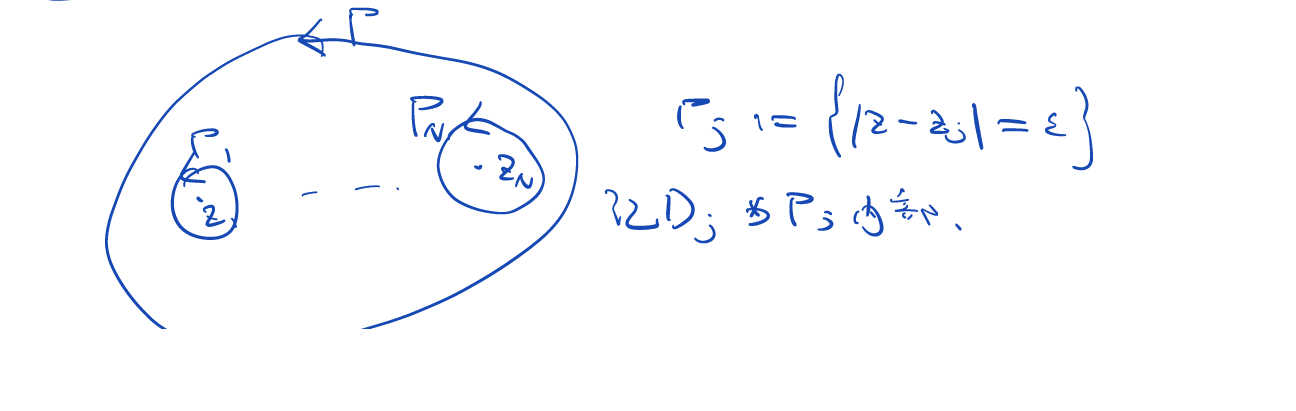
\includegraphics[scale=0.35]{resource/general theta.png}
	\]
	标号分别为$\Gamma_i$和$D_i$.在每个圈内部,我们不妨假设$f=(z-z_i)^{k_j}g_j(z)$
	\begin{align*}
		\frac{f'}{f}=\frac{k_j}{z-z_j}+\frac{g_j'}{g_j}
	\end{align*}
	于是:
	\begin{align*}
		\frac{1}{2\pi \ii}\int_{\Gamma_j}z\frac{f'}{f}dz=k_jz_j(\text{留数定理})
	\end{align*}
\end{proof}
根据引理结论,我们有:
\begin{align*}
	w(z)=\frac{1}{2\pi\ii}\int_{|w-w_0|=\delta}w\frac{\pa{F}{w}}{F}dw
\end{align*}

所以$w$是解析函数.

现在假设$P(z,w)$是二元不可约多项式.(不存在$g,h$使得$P=gh$.)
\begin{theorem}
	$P(z,w)$如上.则至多存在有限个$z \in \C$使得:
    \begin{align*}
		P(z,w)=\pa{P}{w}(z,w)=0 \text{有根}w \in \C
	\end{align*}
\end{theorem}
\begin{proof}
	设$P(z,w)=\sum_{j=0}^n a_j(z)w^j$.因为$P$不可约,则$a_j$没有公共因子。

	设$\pa{P}{w}=\sum_{j=0}^{n}ja_j(z)w^{j-1}=\sum_{j=0}^{n-1}(j+1)a_{j+1}(z)w^j$.于是存在$A_1(z,w)$满足:
	\begin{align*}
		P(z,w)=A_1(z,w)\pa{P}{w}(z,w)+Q_1(z,w) \mathrm{deg}_{w_1}Q_1<\mathrm{deg}_w\pa{P}{w}
	\end{align*}
	
	存在多项式$b_1(z)$满足:
	\begin{align*}
		b_1(z)\pa{P}{w}=A_2(z,w)Q_1(z,w)+Q_2(z,w)
	\end{align*}
    
	\dots

	存在$b_k(z)$满足:
	\begin{align*}
		b_k(z)Q_{k-1}(z,w)=A_{k+1}(z,w)Q_{k}(z,w)+Q_{k+1}(z,w),\mathrm{deg}_{w}Q_{k+1}<\mathrm{deg}_wQ_k
	\end{align*}

	现假设$\mathrm{deg}_w Q_{k+1}(z,w)=0$,即$Q_{k+1}(z,w)\in \C[z]$.我们断言$Q_{k+1}(z)\neq 0$.

	若不然,则$Q_k$的因子可整除$Q_{k-1},\dots,Q_1,\pa{P}{w},P$,与不可约矛盾!

	因而,若$(z_0,w_0)$满足:
	\begin{align*}
		P=\pa{P}{w}=0
	\end{align*}
	则:
	\begin{align*}
		0=Q_1(z_0,w_0)=\dots=Q_{k+1}(z_0)
	\end{align*}
	由于$Q_{k+1}(z)$的零点有限,因而$(z_0,w_0)$也必定是有限的.
\end{proof}

借助上述定理,再结合Implicit Theorem,我们可以发现有趣的事实:

考虑集合$\{(z,w)|P(z,w)=0\}$,这个集合并不一定是黎曼曲面.然而,如果去掉有限个奇异点(即使得方程:
\begin{align*}
		P=\pa{P}{w}=0
	\end{align*}成立的点)后,集合就成为了一个黎曼曲面.

	代数曲线是代数几何中重要的研究对象.
\section{切向量与全纯切丛}
本节我们阐述黎曼曲面的切向量与全纯切丛.如果读者已经学过复几何,这部分可以略过.
\subsection*{切向量与切空间}
由于我们定义黎曼曲面的方式是内蕴的(即没有依靠把$M$“塞进”一个欧氏空间),因而我们也得内蕴的定义黎曼曲面的切向量与切空间.

一个比较自然的想法是,既然黎曼曲面局部上与$\C$的开集等同,并且切空间与切向量看起来也只是局部的几何对象,我们可以借助图卡来定义切空间与切向量.不过这种办法会遇到定义与坐标选取是否有关的问题.

\begin{definition}
	对于黎曼曲面$M$和$p\in M$,$p$处的切向量定义一个为作用在$C^\infty(\{p\})$(即$p$处的光滑函数芽)上的线性算子$V_p$,并且满足:
	\begin{enumerate}
	\item $\forall f \in C^\infty(M),V_p(f)\in \R$
	\item $\forall f,g \in C^\infty(M),V_p(fg)=f(p)V_p(g)+V_p(f)g(p)$
	\end{enumerate}
	所有满足上述条件的线性算子的集合记为$T_p(M)$.
\end{definition}

这里对切向量的定义与微分流形中切向量的定义完全一致,因此我们只罗列切向量的性质,省略掉这些性质的证明.读者请自行查阅微分流形的相关资料.
\begin{proposition}
	$T_pM$是有限维实线性空间,维数为$2$(即$M$的实维数).如果$p$处有局部坐标$(U_\alpha,\varphi_\alpha)$,则$T_pM$有一组基$\{\pa{}{x},\pa{}{y}\}$.其中$x,y$是$\varphi_\alpha$给出的实坐标,并且$\pa{}{x},\pa{}{y}$的定义为:
	\begin{align*}
		\pa{}{x}(f)=\pa{f\circ \varphi_\alpha^{-1}}{x},\pa{}{y}(f)=\pa{f\circ \varphi_\alpha^{-1}}{y}
	\end{align*}
\end{proposition}
\begin{proposition}
	设$T_pM$在两组局部坐标$(U_\alpha,\varphi_\alpha),(U_\beta,\varphi_\beta)$下有两组对应的向量基.则他们的变换公式为:
	\begin{align*}
		\begin{pmatrix}
			\pa{}{x_\beta}\\
			\pa{}{y_\beta}
		\end{pmatrix}=\begin{pmatrix}
			\pa{x_\alpha}{x_\beta}&\pa{y_\alpha}{x_\beta}\\
			\pa{x_\alpha}{y_\beta}&\pa{y_\alpha}{y_\beta}\end{pmatrix}\begin{pmatrix}
				\pa{}{x_\alpha}\\
				\pa{}{y_\alpha}
			\end{pmatrix}
	\end{align*}
	其中$x_\alpha,y_\alpha$是局部的坐标函数,即$x_\alpha=x\circ \varphi_\alpha$,$y_\alpha=y \circ \varphi_\alpha$.
\end{proposition}
\begin{proposition}[切映射]
	考虑两个黎曼曲面的光滑映射(定义与全纯映射类似)$f:M \to N$.$f$可以诱导$T_pM$与$T_{f(p)}N$之间的线性映射$df_p$.定义为:
	\begin{align*}
		\forall g \in C^\infty(\{f(p)\}),df_p(V_p)(g)=V_p(g \circ f)
	\end{align*}

	$df_p$在坐标基的表达式为(只写$x_\alpha$的):
	\begin{align*}
		df_p \pa{}{x_\alpha}=\pa{f^1}{x_\alpha}\pa{}{x_\beta}+\pa{f^2}{x_\alpha}{y_\beta}
	\end{align*}
	其中,$f^1$和$f^2$是$f$在两个局部坐标下的分量形式.(如$f^1=x_\beta \circ f \circ \varphi_\alpha$ )
\end{proposition}
\subsection*{切丛,复切丛}
把$M$上所有的切空间并在一起,用$TM$整体表示这个集合.即:
\begin{align*}
	TM=\bigcup_{p \in M}T_pM
\end{align*}
不难证明,$TM$是一个微分流形,并且维数是$M$的两倍.在我们这里的讨论中,$TM$是一个4维的微分流形,并且自然投射:
\begin{align*}
	\pi:TM \to M,V_p \mapsto p
\end{align*}
是一个光滑映射.
\ifx\allfiles\undefined
	
	% 如果有这一部分的参考文献的话,在这里加上
	% 没有的话不需要
	% 因此各个部分的参考文献可以分开放置
	% 也可以统一放在主文件末尾。
	
	%  bibfile.bib是放置参考文献的文件,可以用zotero导出。
	% \bibliography{bibfile}
	
	\end{document}
	\else
	\fi
\ifx\allfiles\undefined

	% 如果有这一部分另外的package,在这里加上
	% 没有的话不需要
	
	\begin{document}
\else
\fi
\chapter{Morse理论的应用——测地线变分}
\section{道路的能量积分}
\section{指标定理}
\section{道路空间的伦型}


\ifx\allfiles\undefined
	
	% 如果有这一部分的参考文献的话,在这里加上
	% 没有的话不需要
	% 因此各个部分的参考文献可以分开放置
	% 也可以统一放在主文件末尾。
	
	%  bibfile.bib是放置参考文献的文件,可以用zotero导出。
	% \bibliography{bibfile}
	
	\end{document}
	\else
	\fi
\ifx\allfiles\undefined

	% 如果有这一部分另外的package,在这里加上
	% 没有的话不需要
\else
\fi
\chapter{除子与线丛}

\ifx\allfiles\undefined
	
	% 如果有这一部分的参考文献的话,在这里加上
	% 没有的话不需要
	% 因此各个部分的参考文献可以分开放置
	% 也可以统一放在主文件末尾。
	
	%  bibfile.bib是放置参考文献的文件,可以用zotero导出。
	% \bibliography{bibfile}
	
	\end{document}
	\else
	\fi
\end{document}